\documentclass[sigplan,10pt,review,anonymous]{acmart}\settopmatter{printfolios=true,printccs=false,printacmref=false}
\settopmatter{printacmref=false}
\setcopyright{none}
\renewcommand\footnotetextcopyrightpermission[1]{}
\pagestyle{plain}

%% Some recommended packages.
\usepackage{booktabs}   %% For formal tables:
                        %% http://ctan.org/pkg/booktabs
\usepackage{subcaption} %% For complex figures with subfigures/subcaptions
                        %% http://ctan.org/pkg/subcaption


%%%%%%%%%%%%%%%%%%%%%%%%%%%%%%%%%%%%%%%%%%%%%%%%%%%%%%%%%%%%%%%%%%%%%%%
%% Custom definitions
%%%%%%%%%%%%%%%%%%%%%%%%%%%%%%%%%%%%%%%%%%%%%%%%%%%%%%%%%%%%%%%%%%%%%%%

\usepackage{balance}
%\usepackage{url}
\usepackage{enumitem}
\usepackage{hyperref}
\usepackage{listings}
\usepackage{xspace}
\usepackage{cleveref}
\usepackage{multirow}
\usepackage{microtype}
\usepackage{soul,xcolor}
\usepackage{mathpartir}
\usepackage{amsmath,amsthm}
\usepackage[utf8]{inputenc}
\DeclareUnicodeCharacter{2200}{\ensuremath{\forall}} % ∀
\DeclareUnicodeCharacter{2083}{\ensuremath{_3}} % ₃
\DeclareUnicodeCharacter{2102}{\ensuremath{\mathbb{C}}} % ℂ
\DeclareUnicodeCharacter{D7}{\ensuremath{\times}} % ×
\DeclareUnicodeCharacter{2287}{\ensuremath{\supseteq}} % ⊇
\DeclareUnicodeCharacter{2208}{\ensuremath{\in}} % ∈
\DeclareUnicodeCharacter{230A}{\ensuremath{\lfloor{}}} % ⌊
\DeclareUnicodeCharacter{391}{\ensuremath{\Alpha}} % Α
\DeclareUnicodeCharacter{2293}{\ensuremath{\sqcap}} % ⊓
\DeclareUnicodeCharacter{1D502}{\ensuremath{\mathcal{y}}} % 𝔂
\DeclareUnicodeCharacter{395}{\ensuremath{\Epsilon}} % Ε
\DeclareUnicodeCharacter{2297}{\ensuremath{\otimes}} % ⊗
\DeclareUnicodeCharacter{399}{\ensuremath{\Iota}} % Ι
\DeclareUnicodeCharacter{2218}{\ensuremath{\circ}} % ∘
\DeclareUnicodeCharacter{229B}{\ensuremath{?}} % ⊛
\DeclareUnicodeCharacter{211A}{\ensuremath{\mathbb{Q}}} % ℚ
\DeclareUnicodeCharacter{39D}{\ensuremath{\Nu}} % Ν
\DeclareUnicodeCharacter{3A1}{\ensuremath{\Rho}} % Ρ
\DeclareUnicodeCharacter{3A5}{\ensuremath{\Upsilon}} % Υ
\DeclareUnicodeCharacter{22A7}{\ensuremath{\models}} % ⊧
\DeclareUnicodeCharacter{3A9}{\ensuremath{\Omega}} % Ω
\DeclareUnicodeCharacter{2228}{\ensuremath{\lor}} % ∨
\DeclareUnicodeCharacter{3B1}{\ensuremath{\alpha}} % α
\DeclareUnicodeCharacter{B3}{\ensuremath{^3}} % ³
\DeclareUnicodeCharacter{3B5}{\ensuremath{\epsilon}} % ε
\DeclareUnicodeCharacter{3B9}{\ensuremath{\iota}} % ι
\DeclareUnicodeCharacter{3BD}{\ensuremath{\nu}} % ν
\DeclareUnicodeCharacter{1D53E}{\ensuremath{\mathbb{G}}} % 𝔾
\DeclareUnicodeCharacter{3C1}{\ensuremath{\rho}} % ρ
\DeclareUnicodeCharacter{22C3}{\ensuremath{\bigcup}} % ⋃
\DeclareUnicodeCharacter{1D542}{\ensuremath{\mathbb{K}}} % 𝕂
\DeclareUnicodeCharacter{3C5}{\ensuremath{\upsilon}} % υ
\DeclareUnicodeCharacter{1D546}{\ensuremath{\mathbb{O}}} % 𝕆
\DeclareUnicodeCharacter{3C9}{\ensuremath{\omega}} % ω
\DeclareUnicodeCharacter{1D54A}{\ensuremath{\mathbb{S}}} % 𝕊
\DeclareUnicodeCharacter{1D54E}{\ensuremath{\mathbb{W}}} % 𝕎
\DeclareUnicodeCharacter{1D4D3}{\ensuremath{\mathcal{D}}} % 𝓓
\DeclareUnicodeCharacter{1D552}{\ensuremath{\mathbb{a}}} % 𝕒
\DeclareUnicodeCharacter{1D4D7}{\ensuremath{\mathcal{H}}} % 𝓗
\DeclareUnicodeCharacter{1D556}{\ensuremath{\mathbb{e}}} % 𝕖
\DeclareUnicodeCharacter{1D4DB}{\ensuremath{\mathcal{L}}} % 𝓛
\DeclareUnicodeCharacter{1D55A}{\ensuremath{\mathbb{i}}} % 𝕚
\DeclareUnicodeCharacter{1D4DF}{\ensuremath{\mathcal{P}}} % 𝓟
\DeclareUnicodeCharacter{1D55E}{\ensuremath{\mathbb{m}}} % 𝕞
\DeclareUnicodeCharacter{1D4E3}{\ensuremath{\mathcal{T}}} % 𝓣
\DeclareUnicodeCharacter{1D562}{\ensuremath{\mathbb{q}}} % 𝕢
\DeclareUnicodeCharacter{2264}{\ensuremath{\leq}} % ≤
\DeclareUnicodeCharacter{1D4E7}{\ensuremath{\mathcal{X}}} % 𝓧
\DeclareUnicodeCharacter{1D566}{\ensuremath{\mathbb{u}}} % 𝕦
\DeclareUnicodeCharacter{1D4EB}{\ensuremath{\mathcal{b}}} % 𝓫
\DeclareUnicodeCharacter{1D56A}{\ensuremath{\mathbb{y}}} % 𝕪
\DeclareUnicodeCharacter{1D4EF}{\ensuremath{\mathcal{f}}} % 𝓯
\DeclareUnicodeCharacter{2070}{\ensuremath{^0}} % ⁰
\DeclareUnicodeCharacter{1D4F3}{\ensuremath{\mathcal{j}}} % 𝓳
\DeclareUnicodeCharacter{2074}{\ensuremath{^4}} % ⁴
\DeclareUnicodeCharacter{1D4F7}{\ensuremath{\mathcal{n}}} % 𝓷
\DeclareUnicodeCharacter{27F9}{\ensuremath{\Longrightarrow}} % ⟹
\DeclareUnicodeCharacter{1D4FB}{\ensuremath{\mathcal{r}}} % 𝓻
\DeclareUnicodeCharacter{1D4FF}{\ensuremath{\mathcal{v}}} % 𝓿
\DeclareUnicodeCharacter{1D501}{\ensuremath{\mathcal{x}}} % 𝔁
\DeclareUnicodeCharacter{2080}{\ensuremath{_0}} % ₀
\DeclareUnicodeCharacter{2203}{\ensuremath{\exists}} % ∃
\DeclareUnicodeCharacter{2084}{\ensuremath{_4}} % ₄
\DeclareUnicodeCharacter{2309}{\ensuremath{\rceil{}}} % ⌉
\DeclareUnicodeCharacter{210D}{\ensuremath{\mathbb{H}}} % ℍ
\DeclareUnicodeCharacter{392}{\ensuremath{\Beta}} % Β
\DeclareUnicodeCharacter{2115}{\ensuremath{\mathbb{N}}} % ℕ
\DeclareUnicodeCharacter{2294}{\ensuremath{\sqcup}} % ⊔
\DeclareUnicodeCharacter{396}{\ensuremath{\Zeta}} % Ζ
\DeclareUnicodeCharacter{2119}{\ensuremath{\mathbb{P}}} % ℙ
\DeclareUnicodeCharacter{39A}{\ensuremath{\Kappa}} % Κ
\DeclareUnicodeCharacter{211D}{\ensuremath{\mathbb{R}}} % ℝ
\DeclareUnicodeCharacter{39E}{\ensuremath{\Xi}} % Ξ
\DeclareUnicodeCharacter{22A4}{\ensuremath{\top}} % ⊤
\DeclareUnicodeCharacter{2227}{\ensuremath{\land}} % ∧
\DeclareUnicodeCharacter{3A6}{\ensuremath{\Phi}} % Φ
\DeclareUnicodeCharacter{3B2}{\ensuremath{\beta}} % β
\DeclareUnicodeCharacter{3B6}{\ensuremath{\zeta}} % ζ
\DeclareUnicodeCharacter{1D539}{\ensuremath{\mathbb{B}}} % 𝔹
\DeclareUnicodeCharacter{3BA}{\ensuremath{\kappa}} % κ
\DeclareUnicodeCharacter{1D53D}{\ensuremath{\mathbb{F}}} % 𝔽
\DeclareUnicodeCharacter{3BE}{\ensuremath{\xi}} % ξ
\DeclareUnicodeCharacter{1D541}{\ensuremath{\mathbb{J}}} % 𝕁
\DeclareUnicodeCharacter{22C0}{\ensuremath{\bigland}} % ⋀
\DeclareUnicodeCharacter{2243}{\ensuremath{\simeq}} % ≃
\DeclareUnicodeCharacter{3C6}{\ensuremath{\phi}} % φ
\DeclareUnicodeCharacter{1D54D}{\ensuremath{\mathbb{V}}} % 𝕍
\DeclareUnicodeCharacter{1D4D0}{\ensuremath{\mathcal{A}}} % 𝓐
\DeclareUnicodeCharacter{21D2}{\ensuremath{\Rightarrow}} % ⇒
\DeclareUnicodeCharacter{1D555}{\ensuremath{\mathbb{d}}} % 𝕕
\DeclareUnicodeCharacter{1D4D4}{\ensuremath{\mathcal{E}}} % 𝓔
\DeclareUnicodeCharacter{1D559}{\ensuremath{\mathbb{h}}} % 𝕙
\DeclareUnicodeCharacter{1D4D8}{\ensuremath{\mathcal{I}}} % 𝓘
\DeclareUnicodeCharacter{1D55D}{\ensuremath{\mathbb{l}}} % 𝕝
\DeclareUnicodeCharacter{1D4DC}{\ensuremath{\mathcal{M}}} % 𝓜
\DeclareUnicodeCharacter{1D561}{\ensuremath{\mathbb{p}}} % 𝕡
\DeclareUnicodeCharacter{1D4E0}{\ensuremath{\mathcal{Q}}} % 𝓠
\DeclareUnicodeCharacter{1D565}{\ensuremath{\mathbb{t}}} % 𝕥
\DeclareUnicodeCharacter{1D4E4}{\ensuremath{\mathcal{U}}} % 𝓤
\DeclareUnicodeCharacter{27E6}{\ensuremath{\llbracket}} % ⟦
\DeclareUnicodeCharacter{1D569}{\ensuremath{\mathbb{x}}} % 𝕩
\DeclareUnicodeCharacter{1D4E8}{\ensuremath{\mathcal{Y}}} % 𝓨
\DeclareUnicodeCharacter{1D4EC}{\ensuremath{\mathcal{c}}} % 𝓬
\DeclareUnicodeCharacter{1D4F0}{\ensuremath{\mathcal{g}}} % 𝓰
\DeclareUnicodeCharacter{1D4F4}{\ensuremath{\mathcal{k}}} % 𝓴
\DeclareUnicodeCharacter{27F6}{\ensuremath{\longrightarrow}} % ⟶
\DeclareUnicodeCharacter{1D4F8}{\ensuremath{\mathcal{o}}} % 𝓸
\DeclareUnicodeCharacter{207B}{\ensuremath{^{-}}} % ⁻
\DeclareUnicodeCharacter{1D4FC}{\ensuremath{\mathcal{s}}} % 𝓼
\DeclareUnicodeCharacter{2081}{\ensuremath{_1}} % ₁
\DeclareUnicodeCharacter{1D500}{\ensuremath{\mathcal{w}}} % 𝔀
\DeclareUnicodeCharacter{2202}{\ensuremath{\partial}} % ∂
\DeclareUnicodeCharacter{2A06}{\ensuremath{\bigsqcup}} % ⨆
\DeclareUnicodeCharacter{2308}{\ensuremath{\lceil{}}} % ⌈
\DeclareUnicodeCharacter{2291}{\ensuremath{\sqsubseteq}} % ⊑
\DeclareUnicodeCharacter{393}{\ensuremath{\Gamma}} % Γ
\DeclareUnicodeCharacter{2295}{\ensuremath{\oplus}} % ⊕
\DeclareUnicodeCharacter{397}{\ensuremath{\Eta}} % Η
\DeclareUnicodeCharacter{39B}{\ensuremath{\Lambda}} % Λ
\DeclareUnicodeCharacter{39F}{\ensuremath{\Omicron}} % Ο
\DeclareUnicodeCharacter{3A3}{\ensuremath{\Sigma}} % Σ
\DeclareUnicodeCharacter{22A5}{\ensuremath{\bot}} % ⊥
\DeclareUnicodeCharacter{2124}{\ensuremath{\mathbb{Z}}} % ℤ
\DeclareUnicodeCharacter{3A7}{\ensuremath{\Chi}} % Χ
\DeclareUnicodeCharacter{2026}{\ensuremath{\dots}} % …
\DeclareUnicodeCharacter{1F4A9}{\ensuremath{\LaTeX}} % 💩
\DeclareUnicodeCharacter{222A}{\ensuremath{\cup}} % ∪
\DeclareUnicodeCharacter{3B3}{\ensuremath{\gamma}} % γ
\DeclareUnicodeCharacter{3B7}{\ensuremath{\eta}} % η
\DeclareUnicodeCharacter{B9}{\ensuremath{^1}} % ¹
\DeclareUnicodeCharacter{1D538}{\ensuremath{\mathbb{A}}} % 𝔸
\DeclareUnicodeCharacter{3BB}{\ensuremath{\lambda}} % λ
\DeclareUnicodeCharacter{1D53C}{\ensuremath{\mathbb{E}}} % 𝔼
\DeclareUnicodeCharacter{3BF}{\ensuremath{\omicron}} % ο
\DeclareUnicodeCharacter{22C1}{\ensuremath{\biglor}} % ⋁
\DeclareUnicodeCharacter{1D540}{\ensuremath{\mathbb{I}}} % 𝕀
\DeclareUnicodeCharacter{3C3}{\ensuremath{\sigma}} % σ
\DeclareUnicodeCharacter{22C5}{\ensuremath{\cdot}} % ⋅
\DeclareUnicodeCharacter{1D544}{\ensuremath{\mathbb{M}}} % 𝕄
\DeclareUnicodeCharacter{3C7}{\ensuremath{\chi}} % χ
\DeclareUnicodeCharacter{1D54C}{\ensuremath{\mathbb{U}}} % 𝕌
\DeclareUnicodeCharacter{1D4D1}{\ensuremath{\mathcal{B}}} % 𝓑
\DeclareUnicodeCharacter{1D550}{\ensuremath{\mathbb{Y}}} % 𝕐
\DeclareUnicodeCharacter{1D4D5}{\ensuremath{\mathcal{F}}} % 𝓕
\DeclareUnicodeCharacter{1D554}{\ensuremath{\mathbb{c}}} % 𝕔
\DeclareUnicodeCharacter{1D4D9}{\ensuremath{\mathcal{J}}} % 𝓙
\DeclareUnicodeCharacter{1D558}{\ensuremath{\mathbb{g}}} % 𝕘
\DeclareUnicodeCharacter{1D4DD}{\ensuremath{\mathcal{N}}} % 𝓝
\DeclareUnicodeCharacter{1D55C}{\ensuremath{\mathbb{k}}} % 𝕜
\DeclareUnicodeCharacter{1D4E1}{\ensuremath{\mathcal{R}}} % 𝓡
\DeclareUnicodeCharacter{1D560}{\ensuremath{\mathbb{o}}} % 𝕠
\DeclareUnicodeCharacter{1D4E5}{\ensuremath{\mathcal{V}}} % 𝓥
\DeclareUnicodeCharacter{1D564}{\ensuremath{\mathbb{s}}} % 𝕤
\DeclareUnicodeCharacter{27E7}{\ensuremath{\rrbracket}} % ⟧
\DeclareUnicodeCharacter{1D4E9}{\ensuremath{\mathcal{Z}}} % 𝓩
\DeclareUnicodeCharacter{1D568}{\ensuremath{\mathbb{w}}} % 𝕨
\DeclareUnicodeCharacter{1D4ED}{\ensuremath{\mathcal{d}}} % 𝓭
\DeclareUnicodeCharacter{1D4F1}{\ensuremath{\mathcal{h}}} % 𝓱
\DeclareUnicodeCharacter{2192}{\ensuremath{\rightarrow}} % →
\DeclareUnicodeCharacter{1D4F5}{\ensuremath{\mathcal{l}}} % 𝓵
\DeclareUnicodeCharacter{1D4F9}{\ensuremath{\mathcal{p}}} % 𝓹
\DeclareUnicodeCharacter{207A}{\ensuremath{^{+}}} % ⁺
\DeclareUnicodeCharacter{1D4FD}{\ensuremath{\mathcal{t}}} % 𝓽
\DeclareUnicodeCharacter{1D503}{\ensuremath{\mathcal{z}}} % 𝔃
\DeclareUnicodeCharacter{2082}{\ensuremath{_2}} % ₂
\DeclareUnicodeCharacter{2A05}{\ensuremath{\bigsqcap}} % ⨅
\DeclareUnicodeCharacter{2286}{\ensuremath{\subseteq}} % ⊆
\DeclareUnicodeCharacter{230B}{\ensuremath{\rfloor{}}} % ⌋
\DeclareUnicodeCharacter{2292}{\ensuremath{\sqsupseteq}} % ⊒
\DeclareUnicodeCharacter{394}{\ensuremath{\Delta}} % Δ
\DeclareUnicodeCharacter{398}{\ensuremath{\Theta}} % Θ
\DeclareUnicodeCharacter{39C}{\ensuremath{\Mu}} % Μ
\DeclareUnicodeCharacter{3A0}{\ensuremath{\Pi}} % Π
\DeclareUnicodeCharacter{22A2}{\ensuremath{\vdash}} % ⊢
\DeclareUnicodeCharacter{3A4}{\ensuremath{\Tau}} % Τ
\DeclareUnicodeCharacter{2229}{\ensuremath{\cap}} % ∩
\DeclareUnicodeCharacter{3A8}{\ensuremath{\Psi}} % Ψ
\DeclareUnicodeCharacter{B2}{\ensuremath{^2}} % ²
\DeclareUnicodeCharacter{3B4}{\ensuremath{\delta}} % δ
\DeclareUnicodeCharacter{3B8}{\ensuremath{\theta}} % θ
\DeclareUnicodeCharacter{1D53B}{\ensuremath{\mathbb{D}}} % 𝔻
\DeclareUnicodeCharacter{3BC}{\ensuremath{\mu}} % μ
\DeclareUnicodeCharacter{3C0}{\ensuremath{\pi}} % π
\DeclareUnicodeCharacter{1D543}{\ensuremath{\mathbb{L}}} % 𝕃
\DeclareUnicodeCharacter{22C2}{\ensuremath{\bigcap}} % ⋂
\DeclareUnicodeCharacter{2245}{\ensuremath{\cong}} % ≅
\DeclareUnicodeCharacter{3C4}{\ensuremath{\tau}} % τ
\DeclareUnicodeCharacter{3C8}{\ensuremath{\psi}} % ψ
\DeclareUnicodeCharacter{1D54B}{\ensuremath{\mathbb{T}}} % 𝕋
\DeclareUnicodeCharacter{1D54F}{\ensuremath{\mathbb{X}}} % 𝕏
\DeclareUnicodeCharacter{1D553}{\ensuremath{\mathbb{b}}} % 𝕓
\DeclareUnicodeCharacter{1D4D2}{\ensuremath{\mathcal{C}}} % 𝓒
\DeclareUnicodeCharacter{1D557}{\ensuremath{\mathbb{f}}} % 𝕗
\DeclareUnicodeCharacter{1D4D6}{\ensuremath{\mathcal{G}}} % 𝓖
\DeclareUnicodeCharacter{1D55B}{\ensuremath{\mathbb{j}}} % 𝕛
\DeclareUnicodeCharacter{1D4DA}{\ensuremath{\mathcal{K}}} % 𝓚
\DeclareUnicodeCharacter{1D55F}{\ensuremath{\mathbb{n}}} % 𝕟
\DeclareUnicodeCharacter{1D4DE}{\ensuremath{\mathcal{O}}} % 𝓞
\DeclareUnicodeCharacter{2261}{\ensuremath{\equiv}} % ≡
\DeclareUnicodeCharacter{1D563}{\ensuremath{\mathbb{r}}} % 𝕣
\DeclareUnicodeCharacter{1D4E2}{\ensuremath{\mathcal{S}}} % 𝓢
\DeclareUnicodeCharacter{2265}{\ensuremath{\geq}} % ≥
\DeclareUnicodeCharacter{1D567}{\ensuremath{\mathbb{v}}} % 𝕧
\DeclareUnicodeCharacter{1D4E6}{\ensuremath{\mathcal{W}}} % 𝓦
\DeclareUnicodeCharacter{1D56B}{\ensuremath{\mathbb{z}}} % 𝕫
\DeclareUnicodeCharacter{1D4EA}{\ensuremath{\mathcal{a}}} % 𝓪
\DeclareUnicodeCharacter{1D4EE}{\ensuremath{\mathcal{e}}} % 𝓮
\DeclareUnicodeCharacter{1D4F2}{\ensuremath{\mathcal{i}}} % 𝓲
\DeclareUnicodeCharacter{1D4F6}{\ensuremath{\mathcal{m}}} % 𝓶
\DeclareUnicodeCharacter{1D4FA}{\ensuremath{\mathcal{q}}} % 𝓺
\DeclareUnicodeCharacter{1D4FE}{\ensuremath{\mathcal{u}}} % 𝓾

\usepackage{mathtools}
\usepackage{tikz}
\usetikzlibrary{calc,decorations.pathmorphing,shapes}
\usepackage{stmaryrd}

\crefformat{section}{§#2#1#3}
\newtheorem{theorem}{Theorem}
\newtheorem{definition}[theorem]{Definition}

\newenvironment{nop}{}{}
\newenvironment{smathpar}{
\begin{nop}\small\begin{mathpar}}{
\end{mathpar}\end{nop}\ignorespacesafterend}

\newcommand{\kc}[1]{{\color{red} {\it [KC says: #1]}}}
\newcommand{\am}[1]{{\color{blue} {\it [AM says: #1]}}}
\newcommand{\tk}[1]{{\color{blue} {\it [TK says: #1]}}}

\definecolor{Bittersweet}{rgb}{1.0, 0.44, 0.37}
\definecolor{MidnightBlue}{rgb}{0.0, 0.2, 0.4}
\definecolor{BrightBlue}{rgb}{0.0, 0.2, 0.7}
\definecolor{byzantine}{rgb}{0.74, 0.2, 0.64}
\definecolor{caribbeangreen}{rgb}{0.0, 0.8, 0.6}

\lstset{
      language=caml,
      basicstyle=\ttfamily\footnotesize,
      flexiblecolumns=false,
      tabsize=2,
      escapechar={<@}{@>},
      %basewidth={0.5em,0.45em},
      %aboveskip={3pt},
      %belowskip={3pt},
      breaklines = true,
      breakatwhitespace = true,
      keywordstyle=\color{Bittersweet}\bfseries,
      commentstyle=\color{blue}\itshape,
      stringstyle=\color{MidnightBlue},
      keywords=[2]{},
      keywordstyle=[2]\color{byzantine}\bfseries,
      keywords=[3]{eff,effect,perform,continue,discontinue,continuation,
                   clone_continuation},
      keywordstyle=[3]\color{caribbeangreen}\bfseries,
      keywords=[4]{call,return,external},
      keywordstyle=[4]\color{Bittersweet}\bfseries,
      classoffset=1,
      upquote=true,
      keywordstyle=\color{byzantine}\bfseries,
      classoffset=0,
      mathescape=true,
      numberstyle=\tiny\color{gray},
      numbersep=5pt
}

\lstnewenvironment{code}[1][]
    { % \centering
      \lstset{
        basicstyle=\ttfamily\footnotesize,
        #1}%
      \csname lst@setfirstlabel\endcsname}
    { %\centering
      \csname lst@savefirstlabel\endcsname}

\lstMakeShortInline[columns=fullflexible,keepspaces]|

\newcommand{\mycaption}[1]{\vspace{-4mm}\caption{#1}}

%%%%%%%%%%%%%%%%%%%%%%%%%%%%%%%%%%%%%%%%%%%%%%%%%%%%%%%%%%%%%%%%%%%%%%%
%% Semantics definitions
%%%%%%%%%%%%%%%%%%%%%%%%%%%%%%%%%%%%%%%%%%%%%%%%%%%%%%%%%%%%%%%%%%%%%%%


\newcommand{\olam}[2]{\lambda^o #1. #2}
\newcommand{\llambda}{\lambda\!\!\lambda}
\newcommand{\clam}[2]{\lambda^c #1. #2}
\newcommand{\lam}[2]{\Lambda #1. #2}

\newcommand{\env}{\epsilon}
\newcommand{\envext}[3]{#1[#2 \mapsto #3]}

\newcommand{\oclos}[3]{\llparenthesis \olam{#1}{#2}, #3 \rrparenthesis}
\newcommand{\cclos}[3]{\llparenthesis \clam{#1}{#2}, #3 \rrparenthesis}
\newcommand{\clos}[3]{\llparenthesis \lam{#1}{#2}, #3 \rrparenthesis}
\newcommand{\kw}[1]{\text{\bf #1}}
\newcommand{\effval}[2]{\textsf{eff} ~#1 ~#2}
\newcommand{\exnval}[1]{\textsf{exn} ~#1}

\newcommand{\handle}[2]{\kw{match} ~#1 ~\kw{with} ~#2}
\newcommand{\throw}[2]{\kw{raise} ~#1 ~#2}
\newcommand{\perform}[2]{\kw{perform} ~#1 ~#2}

\newcommand{\caseval}[2]{\kw{return}~#1 \mapsto #2}
\newcommand{\caseexn}[3]{\kw{exception} ~#1 ~#2 \mapsto #3}
\newcommand{\caseeff}[4]{\kw{effect} ~#1 ~#2 ~#3 \mapsto #4}

\newcommand{\farg}[2]{\langle #1 ~#2 \rangle_a}
\newcommand{\ffun}[1]{\langle #1 \rangle_f}
\newcommand{\faritha}[3]{\langle #1 ~#2 ~#3 \rangle_{b1}}
\newcommand{\farithb}[2]{\langle #1 ~#2 \rangle_{b2}}

\newcommand{\kcons}{\lhd}
\newcommand{\fiber}{\varphi}
\newcommand{\fl}{\psi} % Frame List
\newcommand{\hc}{\eta} % Handler Closure

\newcommand{\cstack}{\gamma} % C Stack
\newcommand{\ostack}{\omega} % OCaml Stack
\newcommand{\cstacka}[2]{\big \lceil #1, #2 \big \rceil_c} % C stack with arguments
\newcommand{\ostacka}[2]{\big \lceil #1, #2 \big \rceil_o} % OCaml stack with arguments
\newcommand{\ostackemp}{\bullet}
\newcommand{\stack}{\sigma}

\newcommand{\term}{\tau}
\newcommand{\config}{\mathfrak{C}}
\newcommand{\configa}[3]{\|#1,#2,#3\|}

\newcommand{\ostep}{\xrightarrow{o}}
\newcommand{\cstep}{\xrightarrow{c}}
\newcommand{\step}{\rightarrow}

\begin{document}

\title{Retrofitting Effect Handlers onto OCaml}

\begin{abstract}
  Effect handlers have gained immense interest in the recent years as a means
  for modular programming with user-defined effects. The runtime semantics of
  effect handlers is particularly attractive as they allow advanced control
  flow mechanisms such as first-class continuations, generators, async/await,
  coroutines to be composably expressed. In this paper, we present the design,
  a full-fledged implementation and evaluation of effect handlers for OCaml, an
  industrial-strength, multi-paradigm programming language. OCaml tends to be
  widely used for systems programming, and is compatible with program analysis
  tools that inspect the stack such as debuggers and profilers. Retrofitting
  effect handlers onto OCaml is challenging since OCaml does not have any
  non-local control flow mechanisms other than exceptions. Our implementation
  of effect handlers for OCaml imposes negligible overhead on code that does
  not use effect handlers, and remains compatible with program analysis tools
  that inspect the stack.
\end{abstract}

\maketitle

\section{Introduction}

Effect Handlers~\cite{Plotkin09} provide a modular foundation for user-defined
effects. The key idea is to separate the definition of the effectful operations
from their interpretations, which are defined by \emph{handlers} of the
effects. For example,
%
\begin{lstlisting}
effect Read : in_channel -> string
\end{lstlisting}
%
declares an \emph{effect} |Read|, which is parameterised with an input channel
of type |in_channel|, which when \emph{performed} returns a |string| value. A
computation can perform the |Read| effect without knowing how the |Read| effect
is implemented. This computation may be enclosed by different handlers that
interpret |Read| differently. For example, |Read| may be implemented by
performing a blocking read on the input channel or performing the read
asynchronously by offloading it to an event loop such as |libuv|. Thanks to the
separation of effectful operations from their interpretations, effect handlers
enable new approaches to modular programming.

\subsection{An effectful calculator}

What makes effect handlers quite powerful is that they provide a structured
form of delimited continuations~\cite{}, which enables advanced non-local
control-flow mechanisms such as resumable exceptions, coroutines, generators
and asynchronous I/O to be composably expressed. As an example, consider the
task of handling division-by-zero case in a calculator application. Different
calculators handle division-by-zero differently. In the iOS 13 Calculator App
(|iOS|), division-by-zero returns |Error|. In the Google search calculator App
(|gsearch|) |0/0| returns to |Error|, and for any other |n| not equal to |0|,
|n/0| returns |Infinity| with the same sign as |n|. How can we capture these
different behaviours without changing the evaluator?

Common Lisp Conditions~\cite{Conditions} are an elegant way to solve this
problem. Unlike exceptions where the library decides whether an error is fatal
or not, conditions allow the client of the library to make that decision. If
the error is non-fatal, Conditions provide a \emph{restart} mechanism to resume
execution from the point where the condition was signalled. On
division-by-zero, the calculator signals the handler and lets the handler
decide the course of action based on the desired semantics. We can implement
this mechanism using effect handlers as shown below:

\begin{lstlisting}[numbers=left]
type sign = P | N
type val = Z of int | Error | Inf of sign
type exp = Val of val | ... | Div of exp*exp
effect DivBy0 : int -> val
let rec eval e =
  match e with
  | Val v -> v
  | ...
  | Div (e1,e2) ->
    match eval e1, eval e2 with
    | Z v1, Z v2 ->
        if v2 = 0 then perform (DivBy0 v1)
        else Z (v1/v2)
    | Error, _ -> Error | Inf s, _ -> Inf s
    | ...
let (/) n d = Div (Val (Z n), Val (Z d))
\end{lstlisting}

On line 4, we declare an effect |DivBy0| which is parameterised by an integer,
which when performed returns result of division. If the denominator is 0, then
we perform |DivBy0| effect with the numerator value (line 12) so that the
context may decide the return value. We can get the |iOS| semantics by wrapping
the evaluator computation with the following handler:
\begin{lstlisting}
let ios e = match eval e with
| v -> v
| effect (DivBy0 _) k -> continue k Error
\end{lstlisting}
If the evaluator returns a value, we simply return that. In case the evaluator
performs the |DivBy0| effect, we catch the effect in the effect case along with
the continuation |k| of the corresponding |perform| \emph{delimited} by this
handler. In the case of |iOS|, we |continue| the suspended computation with
|Error| value. Hence, the computation |ios(1/0)| returns |Error|. On the
other hand, we can get |gsearch| semantics by enclosing the evaluator in the
following handler:
\begin{lstlisting}
let gsearch e = match eval e with
| v -> v
| effect (DivBy0 v) k ->
  if v = 0 then continue k Error
  else if v > 0 then continue k (Inf P)
  else continue k (Inf N)
\end{lstlisting}
The computation |gsearch(1/0)| returns positive infinity (|Inf P|).

\subsection{Asynchronous I/O}
\label{sec:aio}

We can extend the calculator modularly with the ability to read user input
using the |Read| effect defined earlier as follows:
\begin{lstlisting}
type exp = ... | Inp
effect Read : in_channel -> string
let rec eval e = match e with
| ...
| Inp -> int_of_string(perform(Read stdin))
\end{lstlisting}
The |Read| effect can then be handled by another handler enclosing the
division-by-zero handler:
\begin{lstlisting}
let run e = match gsearch e with
| v -> v
| effect (Read chan) k ->
  register_async_input_line (chan, k);
  continue (get_ui_k ()) ()
\end{lstlisting}
\noindent which registers the read operation to be performed asynchronously
with the continuation as the callback. Subsequently, it resumes the
user-interface continuation so that the application remains responsive. Observe
that neither of the handlers needs to be aware of the other.

\subsection{Retrofitting effect handlers}

There are many research languages and libraries built around effect
handlers~\cite{Koka,Links,Pyro,Frank,Eff}. Unlike these efforts, our goal is to
retrofit effect handlers onto the OCaml programming language, which has been in
continuous use for the past 25 years in large codebases including verification
tools~\cite{FStar,Coq}, mission critical software systems~\cite{astree} and
latency sensitive networked applications~\cite{JS,Docker,MirageOS}. OCaml is
particularly favoured for its competitive yet predictable performance, with
fast foreign-function interface (FFI) and excellent compatibility with program
analysis tools such as debuggers and profilers that utilise DWARF stack unwind
tables~\cite{DWARF} to obtain a backtrace. Our primary motivation for adding
effect handlers to OCaml is to support (1) highly concurrent applications such
as web servers to be expressed naturally in \emph{direct-style} as opposed to
using callbacks and (2) efficient data and task parallel programs in the vein
of Cilk~\cite{}, OpenMP~\cite{} and Intel TBB~\cite{}.

OCaml, however, does not support any non-local control flow mechanisms other
than exceptions. This makes it particularly challenging to implement the
delimited continuations necessary for effect handlers without sacrificing the
desirable properties of OCaml. One standard way of implementing continuations
is to use continuation-passing style (CPS) in the compiler's intermediate
representation (IR)~\cite{Koka}. If the compiler were to use CPS, then reifying
continuations in the source language is relatively straight-forward. But OCaml
does not use CPS IR, and changing the OCaml compiler to utilise CPS IR would be
an enormous undertaking. CPS IR would also affect the performance profile of
OCaml applications due to increased memory allocations as continuation closures
get allocated on the heap~\cite{Folklore}. Moreover, with CPS, stack unwinding
is meaningless and hence, we would lose compatibility with tools that inspect
the program stack. Hence, we choose not to use CPS translation and represent
continuations as call stacks.

The search for an expressive effect system that guarantees that all the effects
performed in the program are handled (\emph{effect safety}) in the presence of
advanced features such as polymorphism, modularity and generativity is an
active area of research~\cite{Leijen14, Biernacki19, Biernacki20,
Hillerstrom20}. We do not focus on this question in this paper, and our
implementation of effect handlers in OCaml does not guarantee effect safety.
For example, running |perform (Read stdin)| without an enclosing handler raises
|Unhandled| exception at the point of |perform|. We leave the question of
effect safety for future work.

\subsection{Requirements}
\label{sec:req}

We motivate our effect handler design based on the following ideal
requirements:

\if{0}
\begin{enumerate}[label=R\arabic*]
  \item \textbf{Backwards compatibility} A well-behaved OCaml program does not
    break under OCaml extended with effect handlers. OCaml code that does not
    use effect handlers will pay negligible performance cost.
  \item \textbf{Tool compatibility} OCaml with effect handlers produce
    well-formed backtraces, and remains compatible with program analysis tools
    such as debuggers and profilers that inspect the stack using DWARF stack
    unwind tables.
  \item \textbf{Effect handler efficiency} In order to support
    highly-concurrent applications, the program must accommodate millions of
    continuations at the same time. Installing effect handlers, capturing and
    resuming continuations must be fast.
  \item \textbf{Forwards compatibility} While this work does not present an
    effect system, the design must be compatible with a future effect system
    for OCaml. As a cornerstone of modularity, we also want blocking I/O code
    to \emph{transparently} be made asynchronous with the help of effect
    handlers.
\end{enumerate}
\fi

\noindent \textbf{R1: Backwards compatibility.} A well-behaved OCaml program does
not break under OCaml extended with effect handlers. OCaml code that does not
use effect handlers will pay negligible performance cost.

\noindent \textbf{R2: Tool compatibility.} OCaml with effect handlers produce
well-formed backtraces, and remains compatible with program analysis tools such
as debuggers and profilers that inspect the stack using DWARF stack unwind
tables.

\noindent \textbf{R3: Effect handler efficiency.} In order to support highly-concurrent
applications, the program must accommodate millions of continuations at the
same time. Installing effect handlers, capturing and resuming continuations
must be fast.

\noindent \textbf{R4: Forwards compatibility.} While this work does not present an
effect system, the design must be compatible with a future effect system for
OCaml. As a cornerstone of modularity, we also want blocking I/O code to
\emph{transparently} be made asynchronous with the help of effect handlers.

The need to host millions of continuations at the same time rules out the use
of large contiguous stack space as in C for continuations. Instead, we resort
to using small initial stacks and growing the stacks on demand. As a result,
OCaml functions, irrespective of whether they use effect handlers, need to
perform stack overflow checks and external C functions, which do not have stack
overflow checks, must be performed on a separate system stack. Additionally, we
must generate DWARF stack unwind tables for stacks that may be non-contiguous.
In this work, we develop the compiler and runtime support for implementing
efficient effect handlers for OCaml that satisfy these requirements.

Our work is also timely. WebAssembly~\ref{} community group is actively
considering effect handlers as one of the mechanism for supporting concurrency,
asynchronous I/O and generators~\ref{WasmPropoal}. Project Loom~\cite{} is an
OpenJDK project which adds virtual threads and delimited continuations to Java.
Swift concurrency roadmap~\cite{} includes direct-style asynchronous
programming and structured concurrency as milestones. We believe that our
design choices will inform similar choices to be made in the other
industrial-strength languages.

\subsection{Contributions}

Our contributions are to present:

\begin{itemize}
  \item the design and implementation of one-shot effect handlers for OCaml.
    Our design retains OCaml's compatibility with program analysis tools that
    inspect the stack using DWARF unwind tables. We have validated our DWARF
    unwind tables using an automated validator tool~\cite{}.
  \item a formal operational semantics for the effect handler implementation in
    OCaml.
  \item extensive evaluation which shows that our implementation has negligible
    impact on code that does not use effect handlers, and serves as an
    efficient foundation for scalable concurrent and parallel programming.
\end{itemize}

We have implemented effect handlers in a multicore extension of the OCaml
programming language. We call our implementation ``Multicore OCaml'' to
distinguish it from stock OCaml.

The rest of the paper is organized as follows. We describe the details of the
OCaml program stack in the next section, and highlight the features that the
effect handler implementation must retain in order to provide backwards
compatibility. In \S\ref{sec:refine}, we refine the design further focussing on
the issues that come up when integrating effect handlers into a mainstream
systems language. \S\ref{sec:semantics} presents the formal operational
semantics for Multicore OCaml effect handlers. \S\ref{sec:impl} discusses the
compiler and the runtime system support for implementing effect handlers.
\S\ref{sec:eval} presents extensive performance evaluation of effect handlers
against the goals set in \S\ref{sec:req}. \S\ref{sec:related} and
\S\ref{sec:conc} present the related work and the conclusions.

\section{Background: OCaml Stacks}
\label{sec:stack}

\begin{figure*}
\begin{minipage}{0.30\linewidth}
  \begin{minipage}{\linewidth}
    \begin{lstlisting}[numbers=left]
external ocaml_to_c
  : unit -> int = "ocaml_to_c"
exception E1
exception E2
let c_to_ocaml () = raise E1
let _ = Callback.register
    "c_to_ocaml" c_to_ocaml
let omain () =
  try (* h1 *)
    try (* h2 *) ocaml_to_c ()
    | with E2 -> 0
  | with E1 -> 42;;
let _ = assert (omain () = 42)
    \end{lstlisting}
    \vspace{-2mm}
    \subcaption{\texttt{meander.ml}}
    \label{code:meander_ml}
  \end{minipage}
  \begin{minipage}{\linewidth}
    \begin{lstlisting}[language=c,numbers=left]
#include <caml/mlvalues.h>
#include <caml/callback.h>

value ocaml_to_c (value unit) {
  caml_callback(*caml_named_value
    ("c_to_ocaml"), Val_unit);
  return Val_int(0);
}
    \end{lstlisting}
    \vspace{-4mm}
    \subcaption{\texttt{meander.c}}
    \label{code:meander_c}
  \end{minipage}
\end{minipage}
%
\begin{minipage}{0.30\linewidth}
  \centering
  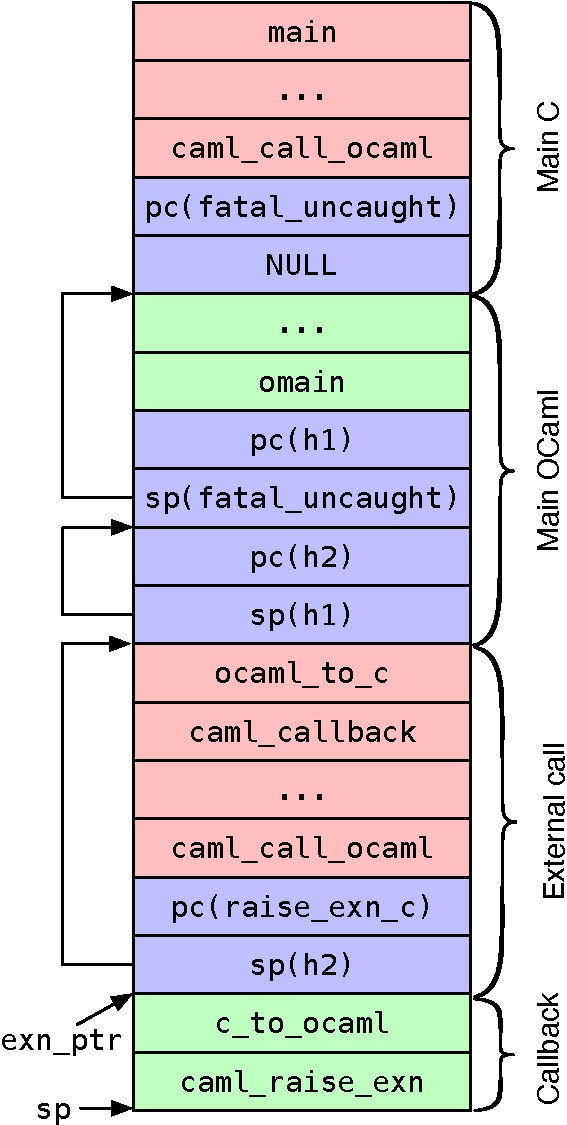
\includegraphics[scale=0.46]{figures/stock_stack}
  \subcaption{Stack layout before raise \texttt{E1}.}
  \label{fig:stock_stack}
\end{minipage}
%
\begin{minipage}{0.39\linewidth}
\begin{lstlisting}[language=c,basicstyle=\ttfamily\footnotesize]
#0  0x925dc in caml_raise_exn ()
#1  0x6fd3e in camlMeander__c_to_ocaml_83 () at meander.ml:5
#2  0x925a4 in caml_call_ocaml ()
#3  0x8a84a in caml_callback_exn (...) at callback.c:145
#4  caml_callback (...) at callback.c:199
#5  0x76e0a in ocaml_to_c (unit=1) at meander.c:5
#6  0x6fd77 in camlMeander__omain_88 () at meander.ml:10
#7  0x6fe92 in camlMeander__entry () at meander.ml:13
#8  0x6f719 in caml_program ()
#9  0x925a4 in caml_call_ocaml ()
#10 0x92e4c in caml_startup_common (...) at startup_nat.c:162
#11 0x92eab in caml_startup_exn (...) at startup_nat.c:167
#12 caml_startup (...) at startup_nat.c:172
#13 0x6f55c in main (...) at main.c:44
\end{lstlisting}
\vspace{-2mm}
\subcaption{\texttt{gdb} backtrace before raise \texttt{E1}.}
\label{code:gdb_backtrace}
\end{minipage}
  \mycaption{Program stack on stock OCaml.}
\end{figure*}

The main challenge in implementing effect handlers in Multicore OCaml is
managing the program stack. To this end, in this section, we provide an
overview of the program stack and related mechanisms in stock OCaml.

In order to illustrate the layout of the stock OCaml stack, consider the
program in Figures~\ref{code:meander_ml} and~\ref{code:meander_c}. The OCaml
main function |omain| installs two exception handlers |h1| and |h2| to handle
exceptions |E1| and |E2|. |omain| calls the external C function |ocaml_to_c|,
which in turn calls back into OCaml function |c_to_ocaml|, which raises the
exception |E1|. OCaml supports raising exceptions in C as well as throwing
exceptions across external calls. Hence, the exception |E1| gets caught in the
handler |h1|, and |omain| returns |42|. The layout of the stack in native code
backend just before raising the exception in |c_to_ocaml| is illustrated in
Figure~\ref{fig:stock_stack}. Note that the stack grows downwards.

OCaml uses the same hardware stack as C, and hence the program stack has
alternating sequences of C and OCaml frames. However, unlike C, OCaml does not
create pointers into OCaml frames. OCaml uses the hardware support for |call|
and |return| instructions for function calls and returns. OCaml does not
perform explicit stack overflow checks in code, and, just like C, relies on the
guard page at the end of the stack region to detect stack overflow. Stack
overflow is detected by a memory fault, and |Stack_overflow| exception is
raised to unwind the stack.

\subsection{External calls and callbacks}
\label{sec:external}

OCaml does not use the C calling convention. In particular, there are no
callee-saved registers in OCaml. On the |x86-64| backend, the C callee-saved
registers, |r15| holds the \emph{allocation pointer} into the minor heap used
for bump pointer allocation, and |r14| holds the |Caml_state|, a table of
global variables used by the runtime. This makes external calls extremely fast
in OCaml. If the external function does not allocate in the OCaml heap, then
the external functions can be called directly, and no bookkeeping is necessary.
For external functions which allocate in the OCaml heap, the cached allocation
pointer is saved to a field in the |Caml_state| before the external call, and
loaded back on return. Similarly, callbacks into OCaml are also cheap.
Callbacks into OCaml involves loading the arguments in the right registers and
calling the OCaml function. OCaml callbacks are relatively common as the
garbage collector (GC) finalisation functions are executed as OCaml callbacks.

\subsection{Exception handlers}
\label{sec:exn_handlers}

The lack of callee-saved registers also makes exception handling fast as there
are no callee-saved registers to be restored when the exception handler runs.
Hence, installing an exception handler simply pushes the program counter (|pc|)
of the handler and the current exception pointer (|exn_ptr| -- a field in
|Caml_state|). At this point, the exception pointer is updated to be the
current stack pointer (|rsp|). This creates a linked-list of exception handler
frames on the stack as shown in Figure~\ref{fig:stock_stack}. Raising an
exception simply sets |rsp| to |exn_ptr|, loads the saved |exn_ptr|, and jumps
to the |pc| of the handler.

% Note |caml_call_ocaml| is |caml_start_program| in ocaml-multicore source

In order to forward exceptions across C frames, the C stub function
|caml_call_ocaml|, which is the entry point for both the main OCaml code and
callbacks into OCaml, pushes an exception handler frame that forwards the
exception to the innermost OCaml exception handler (|raise_exn_c| in
Figure~\ref{fig:stock_stack}), or prints a fatal error (|fatal_uncaught|) if
there are no enclosing handlers. Exceptions are so cheap in OCaml that it is
very common to use them for \emph{local} control flow.

\subsection{Stack unwinding}
\label{sec:unwind}

OCaml generates \emph{stack maps} in order to accurately identify roots on the
stack for assisting GC. For every call point in the program, OCaml compiler
emits the size of the frame and the set of all live registers in the frame
containing pointers into the heap. During a GC, the OCaml stack is walked and
the roots are marked skipping over the C frames.

OCaml also generates precise DWARF unwind information for OCaml, thanks to
which debuggers such as |gdb| and |lldb|, and profilers such as |perf| work
out-of-the-box. For example, for the program in Figures~\ref{code:meander_ml}
and~\ref{code:meander_c}, one could set a break point in |gdb| at
|caml_raise_exn| to get the backtrace in Figuere~\ref{code:gdb_backtrace} which
corresponds to the stack layout in Figure~\ref{fig:stock_stack}.

The same backtrace can also be obtained by using \emph{frame pointers} instead
of DWARF unwind tables. OCaml allows compiling code with frame pointers, but
they are not enabled by default. OCaml stack tends to be deep with small frames
due to the pervasive use of recursive functions, not all of which are
tail-recursive. Hence, the addition of frame pointers can significantly
increase the size of the
stack~\footnote{https://github.com/ocaml/ocaml/issues/5721\#issuecomment-472965549}.
Moreover, not using frame pointers saves two instructions in the function
prologue and epilogue, and makes an extra register (|rbp| on x86) available.
Note that the DWARF unwind information is complementary to the information used
by OCaml to walk the stack for GC.

In summary, the design of effect handlers in OCaml must accommodate these
desirable properties of OCaml with respect to the program stack.

\section{Refining the design}
\label{sec:refine}

In this section, we refine the effect handler design for the OCaml use case.
The primary motivation for adding effect handlers to OCaml is to support
non-local control flow mechanism to implement asynchronous I/O in direct style,
generators and enable task parallelism. These use cases do not resume the
continuations more than once. Hence, our continuations are one-shot, and
resuming the continuation more than once raises |Invalid_argument| exception.
It is well-known that one-shot continuations can be implemented
efficiently~\cite{Bruggeman96RepresentingControl}.

While OCaml permits throwing exceptions across C frames, we do not allow
effects to propagate across C frames as the C frames would become part of the
captured continuation. Managing C frames as part of the continuation is a
complex endeavour~\cite{Daan17Aplas}, and we find that the complexity budget
outweighs the relatively fewer mechanisms enabled by this addition in our
setting.

The interaction of non-local control flow with systems programming is quite
subtle~\cite{TFP17}. Consider the following function that uses blocking I/O
functions from the OCaml standard library to copy data from the input channel
|ic| to the output channel |oc|:
\begin{lstlisting}
let rec copy ic oc =
  try output_string oc ((input_line ic) ^ "\n");
      copy ic oc
  with _ -> (close_in ic; close_out oc)
\end{lstlisting}

The function |input_line| raises |End_of_file| exception on reaching the end of input.
Although not apparent, the code is written in a defensive style to handle other
exceptional cases such as the channels being closed externally. Both
|input_line| and |output_string| raise |Sys_error| exception if the channel is
closed. This function cleanly closes the channels on exceptional cases;
|close_*| functions do nothing if the channel is already closed.

One of our goals(\S\ref{sec:req}) is to make this code transparently
asynchronous. We can define effects for performing the I/O operations  and wrap
them up in functions with the same signature as the one from the standard
library:
\begin{lstlisting}
effect In_line : in_channel -> string
effect Out_str : out_channel -> string -> unit
let input_line ic = perform (In_line ic)
let output_string oc = perform (Out_str oc)
\end{lstlisting}

We can then use a top-level I/O handler similar to the introductory example
(\S\ref{sec:aio}) to discharge the I/O operations asynchronously and resumes
with the result. This handles value return cases, but what about the
exceptional cases |End_of_file| and |Sys_error|? We introduce a |discontinue|
primitive to resume a continuation by raising an exception. In this example, on
reaching the end of file, we would discontinue the continuation of the |copy|
function with |discontinue k End_of_file|, which raises the exception at
|input_line|, and the open channels will be closed.

Program that use resources such as channels are usually written defensively
with the assumption that calling a function will return \emph{exactly once},
either normally or exceptionally. Since effect handlers in Multicore OCaml do
not ensure that all the effects are handled, if the function performs an effect
with no matching handler, then the function \emph{will not return at all}. To
remedy this, when such an effect bubbles up to the top-level, we discontinue
the continuation with |Unhandled| exception so that the exception handlers may
run and clean up the resources.

\section{Semantics}
\label{sec:semantics}

In this section, we formalise the effect handler design in Multicore OCaml.

\subsection{Static semantics}
\label{sec:static_semantics}

As mentioned earlier, effect handlers in Multicore OCaml do not guarantee
effect safety, but only guarantee type safety. Programs without matching effect
handlers are well-typed Multicore OCaml programs. As a result, our static
semantics is simpler than languages that ensure effect
safety~\cite{Links,Koka,Effekt,Frank,HeliumBiernacki}. This is important for
backwards compatibility as our goal is to retrofit effect handlers to a
language with large legacy codebases. Programs that do not use effects remain
well-typed, and those that do compose well with those that don't.

The static semantics of effect handlers in OCaml is captured succinctly by its
API:
\begin{lstlisting}
type 'a eff = ..
type ('a,'b) continuation
val perform: 'a eff -> 'a
val continue: ('a,'b) continuation -> 'a -> 'b
val discontinue: ('a,'b) continuation -> exn -> 'b
(* Internal API *)
type 'a comp = unit -> 'a
type ('a,'b) handler =
{retc: 'a -> 'b;
 effc: 'c.'c eff -> ('c,'b)continuation -> 'b; }
val match_with: 'a comp -> ('a,'b) handler -> 'b
\end{lstlisting}
We introduce an extensible variant type~\cite{} |'a eff| of effect values,
which when performed using the |perform| primitive returns a |'a| value.
Constructors for the value of type |'a eff| are declared using the effect
declarations. For example, the declaration |effect E : string -> int| is
syntactic sugar for adding a new constructor to the variant type
|type _ eff += E : string -> int eff|. We introduce the type
|('a,'b) continuation| of delimited continuations which expect a |'a| value for
resumption and return |'b| value. The continuations may be |continue|d with a
suitably typed value or |discontinue|d with an exception.

For handling the effects, our implementation extends OCaml's |match ... with|
syntax with effect patterns. The expression
\begin{lstlisting}
match e with
| None -> false | Some b -> b
| effect (E s) k1 -> e1 | effect (F f) k2 -> e2
\end{lstlisting}
\noindent is translated to the equivalent of
\begin{lstlisting}
match_with (fun () -> e)
{ retc = (function None -> false | Some b -> b);
  effc = (function
  | (E s) -> (fun k1 -> e1)
  | (F f) -> (fun k2 -> e2)
  | e -> (fun k -> match perform e with
          | v -> continue k v
          | exception e -> discontinue k e)); }
\end{lstlisting}
For the sake of exposition, we introduce a |('a,'b) handler| type. This handler
handles a |'a comp| that returns a |'a| value, and itself returns a |'b| value.
The handler has a return case of type |'a -> 'b|. The effect case |effc|
handles effects of type |'c eff| with |('c,'b) continuation| and returns a
value of type |'b|. The last case in |effc| \emph{reperforms} any unmatched
effect to the outer handler and returns the value and exceptions back to the
original performer. In the implementation, reperfom is implemented as a
primitive to avoid executing code on the resumption path.

\subsection{Dynamic semantics}

\begin{figure*}
  \begin{minipage}[t]{0.49\linewidth}
  \begin{smathpar}
  \begin{array}{rrcl}
    \text{Constants} & n & \coloneqq & ℤ \\
    \text{Abstractions} & \Lambda & \coloneqq & \lambda^o \mid \lambda^c \\
    \text{Expressions} & e & \coloneqq & n \mid x \mid e ~e \mid  \lam{x}{e} \mid e \odot e \mid \throw{l}{e} \\
                       &   & \mid      & \handle{e}{h} \mid \perform{l}{e} \\
    \text{Handlers} & h & \coloneqq & \{\caseval{x}{e}\} \mid \{\caseexn{l}{x}{e}\} \uplus h \\
                   &   & \mid & \{\caseeff{l}{x}{k}{e}\} \uplus h \\
    \text{Values} & v & \coloneqq & n \mid k \mid \clos{x}{e}{\env} \mid \effval{l}{k} \mid \exnval{l} \\
    \text{Frames} & r & \coloneqq & \farg{e}{\env} \mid \ffun{v} \mid \faritha{\odot}{e}{\env} \mid \farithb{\odot}{ℕ} \\
    \text{Environments} & \env & \coloneqq & \emptyset \mid \envext{\env}{x}{v} \\
  \end{array}
  \end{smathpar}
  \end{minipage}
  \begin{minipage}[t]{0.49\linewidth}
  \begin{smathpar}
  \begin{array}{rrcl}
    \text{Handler Closures} & \hc & \coloneqq & (h,\env) \\
    \text{Frame List} & \fl & \coloneqq & [] \mid r :: \fl \\
    \text{Fibers} & \fiber & \coloneqq & (\fl, \hc) \\
    \text{Continuations} & k & \coloneqq & [] \mid \fiber \kcons k \\
    \text{C stacks} & \cstack & \coloneqq & \cstacka{\fl}{\ostack}\\
    \text{OCaml stacks} & \ostack & \coloneqq & \ostacka{k}{\cstack} \mid \ostackemp \\
    \text{Stacks} & \stack & \coloneqq & \cstack \mid \ostack \\
    \text{Terms} & \term & \coloneqq & e \mid v \\
    \text{Configurations} & \config & \coloneqq & \configa{\tau}{\env}{\stack}
  \end{array}
  \end{smathpar}
  \end{minipage}
  \mycaption{Syntax of expressions and configurations}
  \label{sem:syntax}
\end{figure*}

We present the operational semantics for a core language of effect handlers in
Multicore OCaml. The operational semantics intends to faithfully capture the
semantics of Multicore OCaml effect handlers, and to inform an implementation.

\subsubsection{Syntax}

Figure~\ref{sem:syntax} presents the syntax of expressions and configurations.
Our expressions consists of integer constants ($n$), variables ($x$),
abstraction ($\lam{x}{x}$), application ($e~e$), arithmetic expressions ($e
\odot e$) where $\odot$ ranges over $\{+,-,*,/\}$, raising exceptions
($\throw{l}{e}$), performing effects ($\perform{l}{e}$), and handling effects
($\handle{e}{h}$). Abstractions come in two forms: OCaml abstractions
($\lambda^o$) and C abstractions ($\lambda^c$). The handler consists of a
return case ($\caseval{x}{e}$), zero or more exception cases
($\caseexn{l}{x}{e}$) with label $l$, parameter $x$ and body $e$, and zero or
more effect cases ($\caseeff{l}{x}{k}{e}$) with label $l$, parameter $x$,
continuation $k$ and body $e$.

The operational semantics is an extension of a CEK machine
semantics~\cite{Felleisen} for effect handlers, following the abstract machine
semantics of Hillerstrom et al.~\cite{Hillerstrom2020}. The crucial difference
from Hillerstrom et al. is that our stacks are composed of alternating sequence
of OCaml and C stack segments. The program state is captured as configuration
$\config \coloneqq \configa{\tau}{\env}{\stack}$ with the current term $\tau$
under evaluation, its environment $\env$ and the current stack $\stack$. The
term is either an expression $e$ or a value $v$. The value are integer
constants $n$, continuations $k$, closure $\clos{x}{e}{\env}$, effect being
performed $\effval{l}{k}$ and exception being raised $\exnval{l}$. The
environment is a map from variables to values.

The stack $\stack$ is either a C stack ($\cstack$) or an OCaml stack
($\ostack$). Every C stack $\cstacka{\fl}{\ostack}$ consists of a list of
frames $\fl$, and the OCaml stack $\ostack$ under it. Every OCaml stack is
either empty $\ostackemp$ or non-empty $\ostacka{k}{\cstack}$ with the
C stack $\cstack$ under it. Thus, the program stack is an alternating sequence
of C and OCaml stacks terminating with an empty OCaml stack $\ostackemp$. The
frame list $\fl$ is composed of individual frames $r$, which is one of an
argument frame $\farg{e}{\env}$ with the expression $e$ at the argument
position of an application with its environment $\env$, a function frame
$\ffun{v}$ with the value at the function position of an application, and
frames for evaluating the arguments of an arithmetic expression.

Continuations $k$ are either empty $[]$ or non-empty sequence of \emph{fibers}.
A fiber $\fiber \coloneqq (\fl,\hc)$ is a list of frames $\fl$ and a handler
closure $\hc \coloneqq (h,\env)$, which is a pair of handler $h$ and its
environment $\env$.

\subsubsection{Top-level reductions}

The initial configuration for an expression $e$ is
$\configa{e}{\emptyset}{\cstacka{[]}{\bullet}}$, where the environment and the
stack are empty. The top-level reductions
  \begin{mathpar}
    \begin{array}{cc}
      \textsc{StepC} ~
      \inferrule{(\term, \env, \fl, \ostack) \cstep \config}
                {\configa{\term}{\env}{\cstacka{\fl}{\ostack}} \step \config} &
      \textsc{StepO} ~
      \inferrule{(\term, \env, k, \cstack) \ostep \config}
                {\configa{\term}{\env}{\ostacka{k}{\cstack}} \step \config}
    \end{array}
  \end{mathpar}
can be performed by either by taking a C step $\cstep$ or an OCaml step
$\ostep$. Intuitively, this splits the world into executing C code and OCaml
code.

\begin{figure*}
  \begin{smathpar}
    \begin{array}{rrcl}
      \textsc{Var}     & (x,\env, \fl) & \rightsquigarrow
                       & (\env(x), \env, \fl) \\
      \textsc{Arith1}  & (e_1 \odot e_2, \env, \fl) & \rightsquigarrow
                       & (e_1,\env, \faritha{\odot}{e_2}{\env}::\fl) \\
      \textsc{Arith2}  & (n_1, \_, \faritha{\odot}{e_2}{\env}::\fl) & \rightsquigarrow
                       & (e_2, \env, \farithb{\odot}{n_1}::\fl) \\
      \textsc{Arith3}  & (n_2, \env, \farithb{\odot}{n_1}::\fl) & \rightsquigarrow
                       & (\llbracket n_1 \odot n_2 \rrbracket, \env, \fl) \\
      \textsc{App1}    & (e_1 ~e_2, \env, \fl) & \rightsquigarrow
                       & (e_1, \env, \farg{e_2}{\env}::\fl) \\
      \textsc{App2}    & (\lam{x}{e}, \env, \fl) & \rightsquigarrow
                       & (\clos{x}{e}{\env}, \env, \fl) \\
      \textsc{App3}    & (\clos{x}{e_1}{\env_1}, \_, \farg{e_2}{\env_2}::\fl) & \rightsquigarrow
                       & (e_2, \env_2, \ffun{\clos{x}{e_1}{\env_1}}::\fl) \\
      \textsc{Resume1} & (k,\_,\farg{e_1}{\env_1}::\farg{e_2}{\env_2}::\fl) & \rightsquigarrow
                       & (e_1, \env_1, \ffun{k}::\farg{e_2}{\env_2}::\fl) \\
      \textsc{Resume2} & (\clos{x}{e_1}{\env_1}, \_, \ffun{k}::\farg{e_2}{\env_2}::\fl) & \rightsquigarrow
                       & (e_2, \env_2, \ffun{k}::\ffun{\clos{x}{e_1}{\env_1}}::\fl) \\
      \textsc{Perform} & (\perform{l}{e}, \env, \fl) & \rightsquigarrow
                       & (e, \env, \ffun{\effval{l}{[[],(\{\caseval{x}{x}\},\emptyset)]}}::\fl) \\
      \textsc{Raise}   & (\throw{l}{e}, \env, \fl) & \rightsquigarrow
                       & (e, \env, \ffun{\exnval{l}}::\fl)
    \end{array}
  \end{smathpar}
  \vspace{-1mm}
  \mycaption{Administrative Reductions -- $(\term, \env, \fl) \rightsquigarrow (\tau, \env, \fl)$.}
  \label{sem:step}
\end{figure*}
\begin{figure*}
  \begin{smathpar}
    \begin{array}{rrcll}
      \textsc{AdminC}   & (\term,\env,\fl,\ostack) & \cstep
                        & \configa{\term'}{\env'}{\cstacka{\fl'}{\ostack}}
                        & \text{if } (\term,\env,\fl) \rightsquigarrow (\term',\env',\fl') \\
      \textsc{RetToO}   & (v,\env,[],\ostacka{k}{\cstack}) & \cstep
                        & \configa{v}{\env}{\ostacka{k}{\cstack}} \\
      \textsc{CallC}    & (v, \_, \cclos{x}{e}{\env}::\fl, \ostack) & \cstep
                        & \configa{e}{\envext{\env}{x}{v}}{\cstacka{\fl}{\ostack}} \\
      \textsc{Callback} & (v, \_, \oclos{x}{e}{\env}::\fl, \ostack) & \cstep
                        & \configa{e}{\envext{\env}{x}{v}}{\ostacka{k}{\cstacka{\fl}{\ostack}}}
                        & \text{if } k = [[],(\{\caseval{x}{x}\},\emptyset)] \\
      \textsc{ExnFwdO}  & (v, \env, \ffun{\exnval{l}}::\_, \ostacka{(\fl,\hc) \kcons k}{\cstack}) & \cstep
                        & \configa{v}{\env}{\ostacka{(\ffun{\exnval{l}}::\fl,\hc) \kcons k}{\cstack}}
    \end{array}
  \end{smathpar}
  \vspace{-1mm}
  \mycaption{C Reductions -- $(\term, \env, \fl, \ostack) \cstep \config$.}
  \label{sem:cstep}
\end{figure*}


\subsubsection{C reductions}

The C reduction steps are given in Figure~\ref{sem:cstep}. We can take a C step
by taking an administrative reduction step $\rightsquigarrow$. The
administrative reductions are common to both C and OCaml. The rules
\textsc{Var}, \textsc{Arith1}, \textsc{Arith2}, \textsc{App1}, \textsc{App2}
and \textsc{App3} are standard. \textsc{Arith3} performs the arithmetic
operation on the integers ($\llbracket n_1 \odot n_2 \rrbracket$).
\textsc{Raise} pushes an function frame with exception value to indicate that
an exception is being raised. Similarly, \textsc{Perform} pushes a function
frame with an effect value with an empty continuation
$[[],(\{\caseval{x}{x}\},\emptyset)]$ with no captured frames and an empty
handler with an identity return case alone. We shall return to \textsc{Resume1}
and \textsc{Resume2} later.

Continuing with the rest of the C reduction steps, \textsc{CallC} captures the
behaviour of calling a C function. Since the program is currently executing C,
we can perform the call on the current stack. In case the abstraction is an
OCaml abstraction (\textsc{Callback}), we create an OCaml stack with the C
stack as its tail, with the current continuation being empty. This captures the
behaviour of calling back into OCaml from C. \textsc{RetToO} returns a value to
the enclosing OCaml stack. \textsc{ExnFwdO} forwards a raised exception to the
enclosing OCaml stack, unwinding the rest of the frames. This captures the
semantics of raising OCaml exceptions from C.

\subsubsection{OCaml reductions}

\begin{figure*}
  \begin{smathpar}
    \begin{array}{rrcll}
      \textsc{AdminO}   & (\term,\env,(\fl,\hc) \kcons k,\cstack) & \ostep
                        & \configa{\term'}{\env'}{\ostacka{(\fl',\hc) \kcons k}{\cstack}}
                        & \text{if } (\term,\env,\fl) \rightsquigarrow (\term',\env',\fl') \\
      \textsc{RetToC}   & (v, \_, [([],(h,\emptyset))], \cstack) & \ostep
                        & \configa{v}{\env}{\cstack}
                        & \text{if } h = \{\caseval{x}{x}\} \\
      \textsc{RetFib} & (v, \_, ([],(h,\env)) \kcons k, \cstack) & \ostep
                        & \configa{e}{\envext{\env}{x}{v}}{\ostacka{k}{\cstack}}
                        & \text{if } \{\caseval{x}{e}\} \in h \\
      \textsc{CallO}    & (v, \_, (\oclos{x}{e}{\env}::\fl,\hc) \kcons k, \cstack) & \ostep
                        & \configa{e}{\envext{\env}{x}{v}}{\ostacka{(\fl,\hc) \kcons k}{\cstack}} \\
      \textsc{ExtCall}  & (v, \_, (\cclos{x}{e}{\env}::\fl,\hc) \kcons k, \cstack) & \ostep
                        & \configa{e}{\envext{\env}{x}{v}}{\cstacka{[]}{\ostacka{(\fl,\hc) \kcons k}{\cstack}}} \\
      \textsc{Resume}   & (v, \_, (\ffun{k}::\ffun{\oclos{x}{e}{\env}}::\fl,\hc) \kcons k, \cstack) & \ostep
                        & \configa{e}{\envext{\env}{x}{v}}{\ostacka{k ~@~ ((\fl,\hc) \kcons k')}{\cstack}} \\
      \textsc{Handle}   & (\handle{e}{h}, \env, k, \cstack) & \ostep
                        & \configa{e}{\env}{\ostacka{([],(h,\env)) \kcons k}{\cstack}} \\
      \textsc{EffUnHn}  & (v, \_, [\ffun{\effval{l}{k}}::\fl,(h,\env)], \cstack) & \ostep
                        & \configa{e}{\emptyset}{\ostacka{k ~@~ [(\fl,(h,\env))]}{\cstack}}
                        & \text{if } \{\caseeff{l}{\_}{\_}{\_}\} \notin h \\
                  & & & & \text{and } {e = \throw{\textsf{unhandled}}{0}} \\
      \textsc{EffHn}    & (v, \_, (\ffun{\effval{l}{k}}::\fl,(h,\env)) \kcons k', \cstack) & \ostep
                        & \configa{e}{\env[r \mapsto k''][x \mapsto v]}{\ostacka{k'}{\cstack}}
                        & \text{if } \{\caseeff{l}{x}{r}{e}\} \in h \\
                  & & & & \text{and } k'' = k ~@~ [(\fl,(h,\env))] \\
      \textsc{EffFwd}   & (v, \env', (\ffun{\effval{l}{k}}::\fl,(h,\env)) \kcons (\fl',\hc') \kcons k', \cstack) & \ostep
                        & \configa{v}{\env'}{\ostacka{(\ffun{\effval{l}{k''}}::\fl',\hc') \kcons k'}{\cstack}}
                        & \text{if } \{\caseeff{l}{\_}{\_}{\_}\} \notin h \\
                  & & & & \text{and } k'' = k ~@~ [(\fl,(h,\env))] \\
      \textsc{ExFwdC}   & (v, \env, [\ffun{\exnval{l}}::\_,(h,\_)], \cstacka{\fl'}{\ostack}) & \ostep
                        & \configa{v}{\env}{\cstacka{\ffun{\exnval{l}}::\fl'}{\ostack}}
                        & \text{if } \{\caseexn{l}{\_}{\_}\} \notin h \\
      \textsc{ExHn}     & (v, \_, (\ffun{\exnval{l}}::\_,(h,\env)) \kcons k', \cstack) & \ostep
                        & \configa{e}{\envext{\env}{x}{v}}{\ostacka{k'}{\cstack}}
                        & \text{if } \{\caseexn{l}{x}{e}\} \in h \\
      \textsc{ExFwdFib} & (v, \env, (\ffun{\exnval{l}}::\_,(h,\_)) \kcons (\fl',\hc') \kcons k', \cstack) & \ostep
                        & \configa{v}{\env}{\ostacka{(\ffun{\exnval{l}}::\fl',\hc') \kcons k'}{\cstack}}
                        & \text{if } \{\caseexn{l}{\_}{\_}\} \notin h \\
    \end{array}
  \end{smathpar}
  \vspace{-1mm}
  \mycaption{OCaml Reductions -- $(\term, \env, k, \cstack) \ostep \config$.}
  \label{sem:ostep}
\end{figure*}

In OCaml (Figure~\ref{sem:ostep}), reductions always occur on the top-most
fiber in the current stack. \textsc{AdminO} performs administrative reductions.
\textsc{CallO} evaluates an OCaml function on the current stack.
\textsc{ExtCall} captures the behaviour of external calls, which are evaluated
on an empty C stack. \textsc{RetToC} returns a value to the enclosing C stack.
In this case, we have exactly one fiber on the stack, and this was created in
the rule \textsc{Callback}, whose handler has identity return case alone and
the environment is empty. \textsc{RetFib} returns value from a fiber to the
previous one, evaluating the body of the return case.

The rule \textsc{Handle} installs a handler by pushing a fiber with no frames
and the given handler. The rule \textsc{ExHn} handles an exception, if the
current handler has a matching exception case, unwinding the current fiber. The
rule \textsc{ExFwdC} forwards the exception to C. Here, there is exactly one
fiber on the current stack, and the handler does not have a matching exception
case, which we know is the case (see \textsc{Callback} rule). The rule
\textsc{ExFwdFib} forwards the exception to the next fiber if the current
handler does not handle it.

The rule \textsc{EffHn} captures the handling of effects when the current
handler has a matching effect case. We evaluate the body of the matching case,
and bind the continuation parameter |r| to the captured continuation. Observe
that the captured continuation |k''| includes the current handler. Intuitively,
the handler wraps around captured continuation. This gives Multicore OCaml
effect handlers deep handler semantics~\cite{}. \textsc{EffFwd} forwards the
effect to the outer fiber, and extends the captured continuation |k''| in the
process. Recall that we do not capture C frames as part of a continuation. To
this end, \textsc{EffUnHn} models unhandled effect. If the effect bubbles up to
the top fiber, which we know does not have an effect case (see
\textsc{Callback} rule), we raise \textsc{unhandled} exception at the point
where the corresponding effect was performed. This is achieved by appending the
captured continuation to the front of the current continuation.

Observe that |continue| and |discontinue| are not part of the expressions. They
are encoded as follows: $\textsf{continue} ~k ~e = (k ~(\olam{x}{x})) ~e$ and
$\textsf{discontinue} ~k ~l ~e = (k ~(\olam{x}{\throw{l}{x}})) ~e$.
Intuitively, resuming a continuation in both the cases involves evaluating the
appropriate abstraction on top of the continuation. We perform the
administrative reductions \textsc{Resume1} and \textsc{Resume2} to evaluate the
arguments to |continue| and |discontinue|. The rule \textsc{Resume} appends the
given continuation to the front of the current continuation, and evaluates the
body of the closure.

The traces of example programs are included in the supplementary material along
with an executable version of the semantics implemented in OCaml.

\section{Implementation}
\label{sec:impl}

In this section, we present the implementation details of effect handlers in
Multicore OCaml. The implementation follows the operational semantics, but has
a few key representational differences. Multicore OCaml currently only supports
the x86-64 backend on Linux, but our design does not preclude other backends.
We assume x86-64 architecture in the sequel.

Unlike the operational semantics, handlers with just exception patterns
(exception handlers) are implemented differently from effect handlers. As
mentioned in \S~\ref{sec:exn_handlers}, exceptions are pervasive in OCaml and
are so cheap that they are used for local control flow. Hence, we retain the
linked exception handler frame implementation of stock OCaml exception handlers
in Multicore OCaml for performance backwards compatibility. This differs from
other research languages with effect handlers~\cite{Links,Frank,Eff}, which
implement exceptions using effects (by ignoring the continuation argument in
the handler).

\subsection{Heap-allocated fibers}

\begin{figure*}
\begin{minipage}{0.35\linewidth}
  \centering
  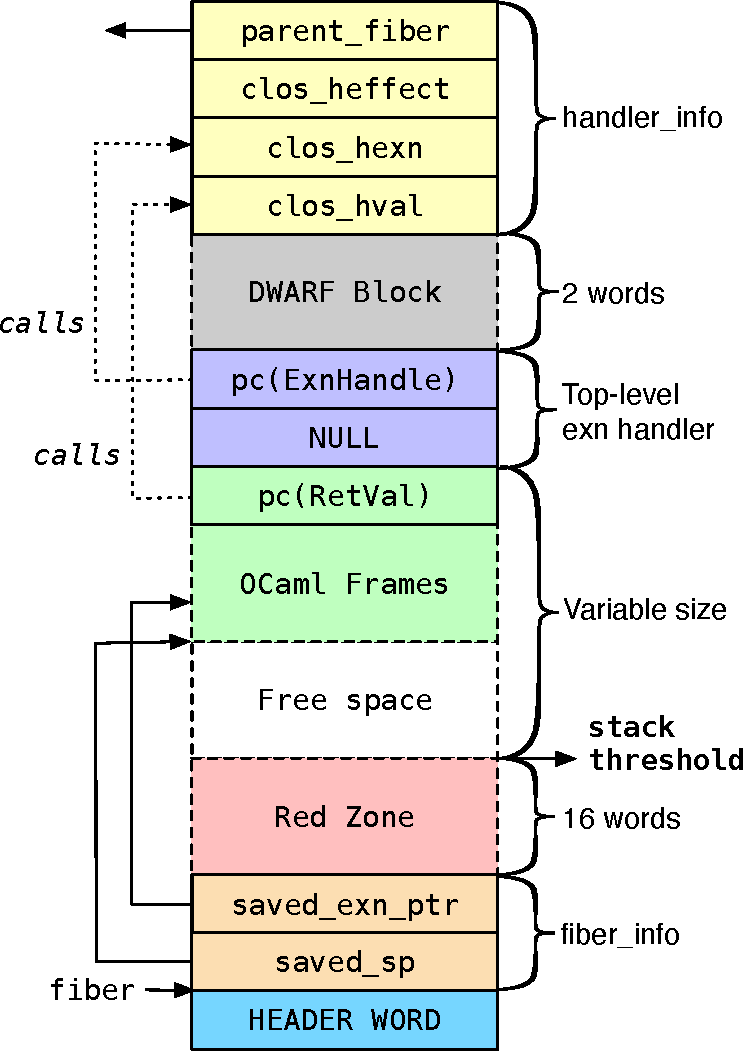
\includegraphics[scale=0.45]{figures/fiber}
  \subcaption{Fiber layout}
  \label{fig:fiber}
\end{minipage}
\begin{minipage}{0.64\linewidth}
  \begin{minipage}{\linewidth}
    \centering
    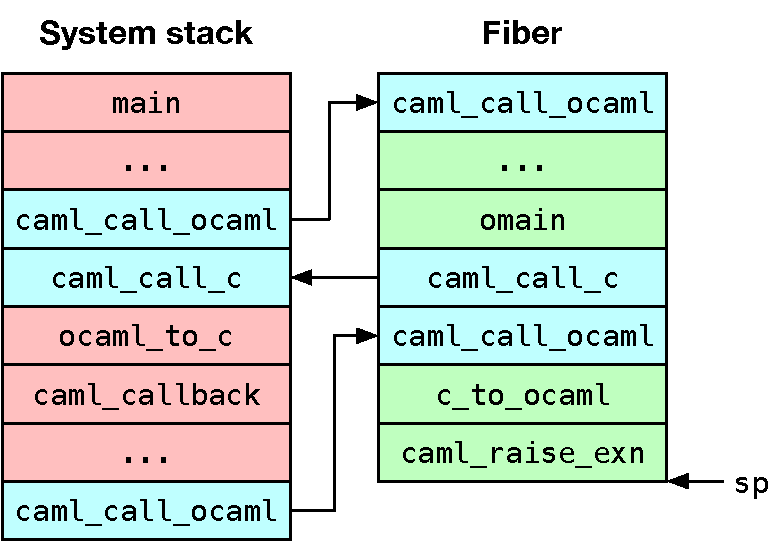
\includegraphics[scale=0.4]{figures/multicore_stack}
    \subcaption{Stack layout for \texttt{meander} example from \S\ref{sec:stack}.}
    \label{fig:mcstack}
    \vspace{2mm}
  \end{minipage}
  %
  \begin{minipage}{0.55\linewidth}
    \begin{lstlisting}
effect E : unit
effect F : unit;;
match (* comp_e *)
  match (* comp_f *)
    (*p1*) perform E (*p3*)
  with | v -> v | effect F kf -> ...
with | v -> v
		 | effect E ke ->
		     (*p2*) continue ke ()
    \end{lstlisting}
		\subcaption{Constructing continuation objects}
		\label{code:effimpl}
  \end{minipage}
  %
  \begin{minipage}{0.44\linewidth}
    \centering
    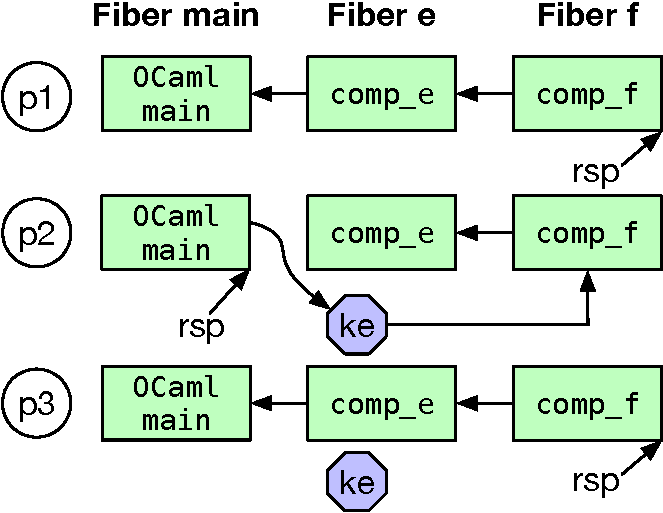
\includegraphics[scale=0.42]{figures/fiber_handler}
		\subcaption{Program state for Figure~\ref{code:effimpl}}
    \label{fig:fiber_handler}
  \end{minipage}
\end{minipage}
\vspace{2mm}
\mycaption{Layout of Multicore OCaml effect handlers.}
\end{figure*}

In the operational semantics, the continuations may be resumed more than once.
Captured continuations are copies of the original fibers and resuming the
continuation copies the fibers and leaves the continuation as it is. In our use
cases, continuations will be resumed at-most once, and copying fibers is
unnecessary and inefficient. Instead, Multicore OCaml allocates fibers on the
heap. Figure~\ref{fig:fiber} shows the layout of a fiber in Multicore OCaml.

At the bottom of the stack, we have the |handler_info|, which contains the
pointer to parent fiber, and the closures for the value, exception and effect
cases. The closures are created by the translation described in
\S\ref{sec:static_semantics}; Multicore OCaml supports exception patterns in
addition to effect patterns in the same handler. This is followed by a block to
support DWARF unwinding, whose details we will return to later. Then, there is
a top-level handler that invokes the exception handler closure |clos_hexn|
after switching to the parent fiber. This is followed by the |pc| of the code
that invokes value handler |clos_hval| after switching to the parent stack. The
stack is laid out such that when the computation in the handler returns,
control goes to value handler.

We have the variable-sized area for the OCaml frames next. Since we want the
handlers to be as small as possible, this area is initially 16 words in length.
When the stack pointer |rsp| goes less than stack threshold (maintained in the
|Caml_state| table), the stack is said to have overflown. On stack overflow, we
copy the whole fiber to a new area with double the size. In Multicore OCaml, we
introduce stack overflow checks into the function prologue of OCaml functions.
We observed that most function calls are to leaf functions with small frame
size. In order to take advantage of this fact, we introduce a small red zone at
the top of the stack. The compiler elides the stack overflow check for leaf
functions whose frame size is less than the size of the red zone.

Finally, we have the saved exception pointer, which points to the top-most
exception frame, and the saved stack pointer, which points to the top of the
stack. Switching between fibers only involves saving the exception and the
stack pointer of the current stack and loading the same on the target stack.
Since OCaml does not generate pointers into the stack, the two |fiber_info|
fields are the only ones that need to be updated when fibers are moved. We
allocate the space for the fiber using |malloc| and |free| it when no longer
required. We do not use a \emph{stack cache} of recently freed stacks for
speeding up fiber allocation~\ref{Farvardin}. In our experiments, we observed
that directly using |mimalloc| outperforms having the stack cache.

\subsection{External calls and callbacks}

Since C functions do not have stack overflow checks, we have to execute the
external calls in the system stack. Calling a C function from OCaml involves
saving the exception and stack pointers in the current fiber, saving the
allocation pointer in the |Caml_state|, updating |rsp| to the top of system
stack (maintained in |Caml_state|), and calling the C function. The actions are
reversed when returning from the external call. One subtlety is that for C
functions that take arguments on the stack, the arguments must be copied to the
C stack from the OCaml stack where they are laid out. For vast majority of
external calls, we perform only a few additional instructions over stock OCaml.

When we first enter OCaml from C, a new fiber is allocated for the main OCaml
stack. Since callbacks may be frequent in OCaml programs that use finalisers,
we run the callbacks on the same fiber as the current one. For example, the
layout of the Multicore OCaml stack at |caml_raise_exn| in the |meander|
example from \S\ref{sec:stack} is shown in Figure~\ref{fig:mcstack}. The
functions |caml_call_c| and |caml_call_ocaml| switch the stacks, and hence are
shown in both the system stack and the fiber. The details of the exception
frames have been elided in the figure. Thanks to the fiber representation,
external calls and callbacks remain fast.

\subsection{Effect handlers}
\label{sec:effimpl}

In order to illustrate the implementation of handling effects, consider the
example presented in Figure~\ref{code:effimpl}. The layout of the program state
as the program executes is captured in Figure~\ref{fig:fiber_handler}. The code
performs |E| which is handled in the outer-most handler, and is immediately
resumed. The arrows between the fibers are parent pointers. At position |p1|,
|rsp| is at the top of the fiber |f|.

When the effect |E| performed, we allocate a continuation object |ke| in the
heap that points to the current fiber |f|, set fiber |f|'s parent pointer to
|NULL|, and evaluate the continuation closure |clos_heffect| on the parent
fiber |e| with the effect |E| and the continuation |ke| as arguments. Since the
first handler does not handle effect |E|, the effect is \emph{reperformed}
(\S\ref{sec:static_semantics}) by appending the fiber |e| to the tail of
continuation |ke|, set fiber |e|'s parent pointer to |NULL|, and evaluate the
current continuation closure on the parent fiber |main| with |E| and |ke| as
arguments, which handles |E| (position |p2|). Thus, continuations are captured
without copying frames. Since every handler closure is evaluated until a
machine one is found, the time taken to handle an effect is linear in the
number of handlers. We observe that the handler stack is shallow in real
programs.

When the continuation is resumed, we overwrite the value of |ke| to |NULL| to
enforce at-most once semantics. Resuming a continuation involves traversing the
linked-list of fibers and making the last fiber point to the current fiber.
Just as in the operational semantics, the implementation invokes the
appropriate closure to either |continue| or |discontinue| the continuation
(position |p3|). We perform standard tail-call optimization so that resumptions
at tail positions do not build up stack.

\subsection{Stack unwinding}

The challenge with DWARF stack unwinding is to make it aware of the
non-contiguous stacks. While the complete details of DWARF stack unwinding is
beyond the scope of the paper, it is beneficial to know how DWARF unwind tables
are constructed in order to appreciate our solution. We refer the interested
reader to Bastian et al.~\cite{} for a good overview of DWARF stack unwinding.

Logically, DWARF maintains a large table which records for every machine
instruction where the return address and callee-saved registers are stored. To
avoid reifying this large table, DWARF represents the table using a compact,
turing-complete, bytecode representation, which is interpreted on demand for
building the stack unwind table. Within each function, DWARF maintains a
\emph{canonical frame address} (CFA), which is invariant in the function body,
and is traditionally the stack pointer before entering this function. Hence, on
x86-64, where the return address is pushed on the stack on call, the return
address is at |CFA - 8|.

Our goal is to help DWARF identify the CFA when stacks are switched at external
calls, callbacks and effect handlers. We have implemented short, hand-written
DWARF bytecode at these three places, which we have validated with the DWARF
unwind table validator tool~\cite{Bastian}. When starting to run on a new
fiber, we insert DWARF bytecode to follow the |parent_fiber| pointer and
dereference the |saved_sp| to get the CFA (|saved_sp + 8|). During callback, we
save the current system stack pointer in the |DWARF block| in
Figure~\ref{fig:fiber} to identify the CFA in the C stack. DWARF unwinding for
external calls is implemented similarly by saving the current OCaml stack
pointer. With these changes, we get the same backtrace for the \texttt{meander}
program from \S\ref{sec:unwind}, modulo runtime system functions due to effect
handlers.

\subsection{Garbage collection}

Recall that OCaml programs are written with the expectation that function calls
return exactly once (\S\ref{sec:refine}). Consider the scenario when a
continuation is neither |continue|d nor |discontinue|d. Since fibers are
|malloc|ed and are |free|d when the computation being handled returns a value
or raises an exception, not resuming continuations leaks memory. In addition,
unresumed continuations may also leak other resource such as open file
descriptors.

We consider well-behaved Multicore OCaml programs to resume their continuations
\emph{exactly once}. This can be enforced by installing a finaliser on every
captured continuation that |discontinue|s the continuation during finalisation
and ignores the result:
\begin{lstlisting}
Gc.finalise (fun k ->
  try ignore (discontinue k Unwind) | _ -> ()) k
\end{lstlisting}
Multicore OCaml does not enforce this behaviour in order to minimise the cost
of using effect handlers.

For stack walking during GC, the only change necessary was to make the runtime
aware of fiber layout and how to follow the parent pointers. The stack map
generation and scanning each frame for roots remains the same. Sivaramakrishnan
et al.~\cite{RetroParallel} present the challenges and solutions for
integrating fibers with the concurrent mark-and-sweep GC of Multicore OCaml.

\section{Evaluation}
\label{sec:eval}

\subsection{The impact on code not using effects}

There are several changes to the runtime to support fibers and effect handlers
that will be executed by code not using effects: OCaml stacks now have dynamic
checks in the function prologue and the FFI interface tracks stack switching.

TODO:
\begin{itemize}
\item Aim: |R1| not altered existing code performance too much
\item sandmark macro benchmarks to show sequential performance: 4.10.0+stock, 4.10.0+multicore,
4.10.0+multicore no red-zone/leaf-optimization, 4.10.0+multicore
\item do we want to include some micro-benchmarks focusing on the FFI callstack overhead?
\end{itemize}

\subsection{Measurements of overheads in our effects implementation}

We have implemented effects within OCaml, here we present timing measurements
for the various stages of stack creation (|a| to |b|), performing and handling
an effect (|b| to |c|), continuation resumption (|c| to |d|) and returning from
a computation and freeing the stack (|d| to |e|).

\begin{lstlisting}
let foo () =
 (* a *) match
 (* b *)   perform E
 (* d *) with effect E k ->
 (* c *)   continue k ()
 (* e *)
\end{lstlisting}

TODO:
\begin{itemize}
\item Aim: |R3| to provide some timing information as to the size of the overhead and where the overhead is.
\item use KC's measurement stubs as presented in WASM
\end{itemize}

\subsection{Effects benchmarks}

We now look at the impact of the overhead in a variety of benchmarks comparing
the cost of using our effects abstraction versus alternative methods of
implementation.

TODO:
\begin{itemize}
\item Aim: |R3| Do we have an efficient implementation of effects and are effects competitive vs alternative implementation strategies.
\item we can show the sequential vs stack benchmarks as used by 'Folklore to fact' \tk{slightly weak story as the sequential ones will be much faster for these very simple benchmarks and effects don't really add anything to their implementation}
\item general generator examples (using examples from effects-example)
\item chamenos vs chamenos effects vs lwt (using examples from effects-example)
\end{itemize}

\subsection{Webserver benchmarks}

TODO:
\begin{itemize}
\item Aim: |R3| Do we have an efficient implementation of effects.
\item effects are a very nice way to program non-blocking IO for webservers
\item show that using effects doesn't impose undue overhead and that we are competitive with LWT, Async, Go with the wrk web benchmark
\end{itemize}


\subsection{Using fibers for task based parallelism}

TODO:
\begin{itemize}
\item Aim: |R3| Do we have an efficient implementation of effects.
\item minor alteration to domainslib to launch tasks in their own stack
\item effects are the right way to do some task base parallelism. Use the nqueens example and show the scaling we can achieve in parallel
\item show that using fibers doesn't have large detrimental impact to existing parallel applications: Take sandmark: minilight, nbody, LU decomposition
\end{itemize}


\section{Related Work}
\label{sec:related}

\section{Conclusions and Future Work}
\label{sec:conc}

\bibliographystyle{ACM-Reference-Format}
\bibliography{sample-base}


\end{document}
